\section{Propuesta de Metodología}\label{sec:propuesta-metodologia}

Esta sección introduce una metodología innovadora que integra el análisis explicativo de SHAP (Shapley Additive Explanations) con el análisis de causalidad de DoWhy, proporcionando un enfoque robusto y detallado para identificar las variables más relevantes y luego construir un modelo causal efectivo. La metodología propuesta se denomina \textit{Análisis Causal Asistido por Minería de Datos} (ACAMD).

\subsection{Beneficios de SHAP y DoWhy}\label{subsec:beneficios-shap-dowhy}

SHAP y DoWhy son herramientas poderosas en el campo del análisis de datos, especialmente cuando se utilizan en conjunto. SHAP ayuda a desentrañar la contribución de cada característica en los modelos predictivos, ofreciendo una comprensión clara de qué variables son las más influyentes. Por otro lado, DoWhy facilita la construcción de modelos causales, permitiendo a los investigadores ir más allá de la correlación y adentrarse en la causalidad.

La integración de SHAP y DoWhy en una sola metodología ofrece varios beneficios. Primero, permite una selección más informada de variables relevantes para el análisis causal, basada en la contribución cuantificable de cada característica. Segundo, proporciona un marco sólido para validar la importancia de estas características en el contexto de los modelos causales. Finalmente, esta combinación promueve un entendimiento más profundo y explicaciones más intuitivas de los fenómenos observados.

\subsection{Proceso de la Metodología ACAMD}\label{subsec:proceso-metodologia}

El proceso de \textit{Análisis Causal Asistido por Minería de Datos} se inicia con la minería de datos, donde se preparan y procesan los datos para el análisis. A continuación, se utiliza SHAP para identificar las características más relevantes, basándose en su impacto en el modelo predictivo. Estas características clave se convierten entonces en el foco del análisis causal con DoWhy, que construye un modelo causal para entender las relaciones subyacentes entre las variables.

\begin{figure}[H]
    \centering
    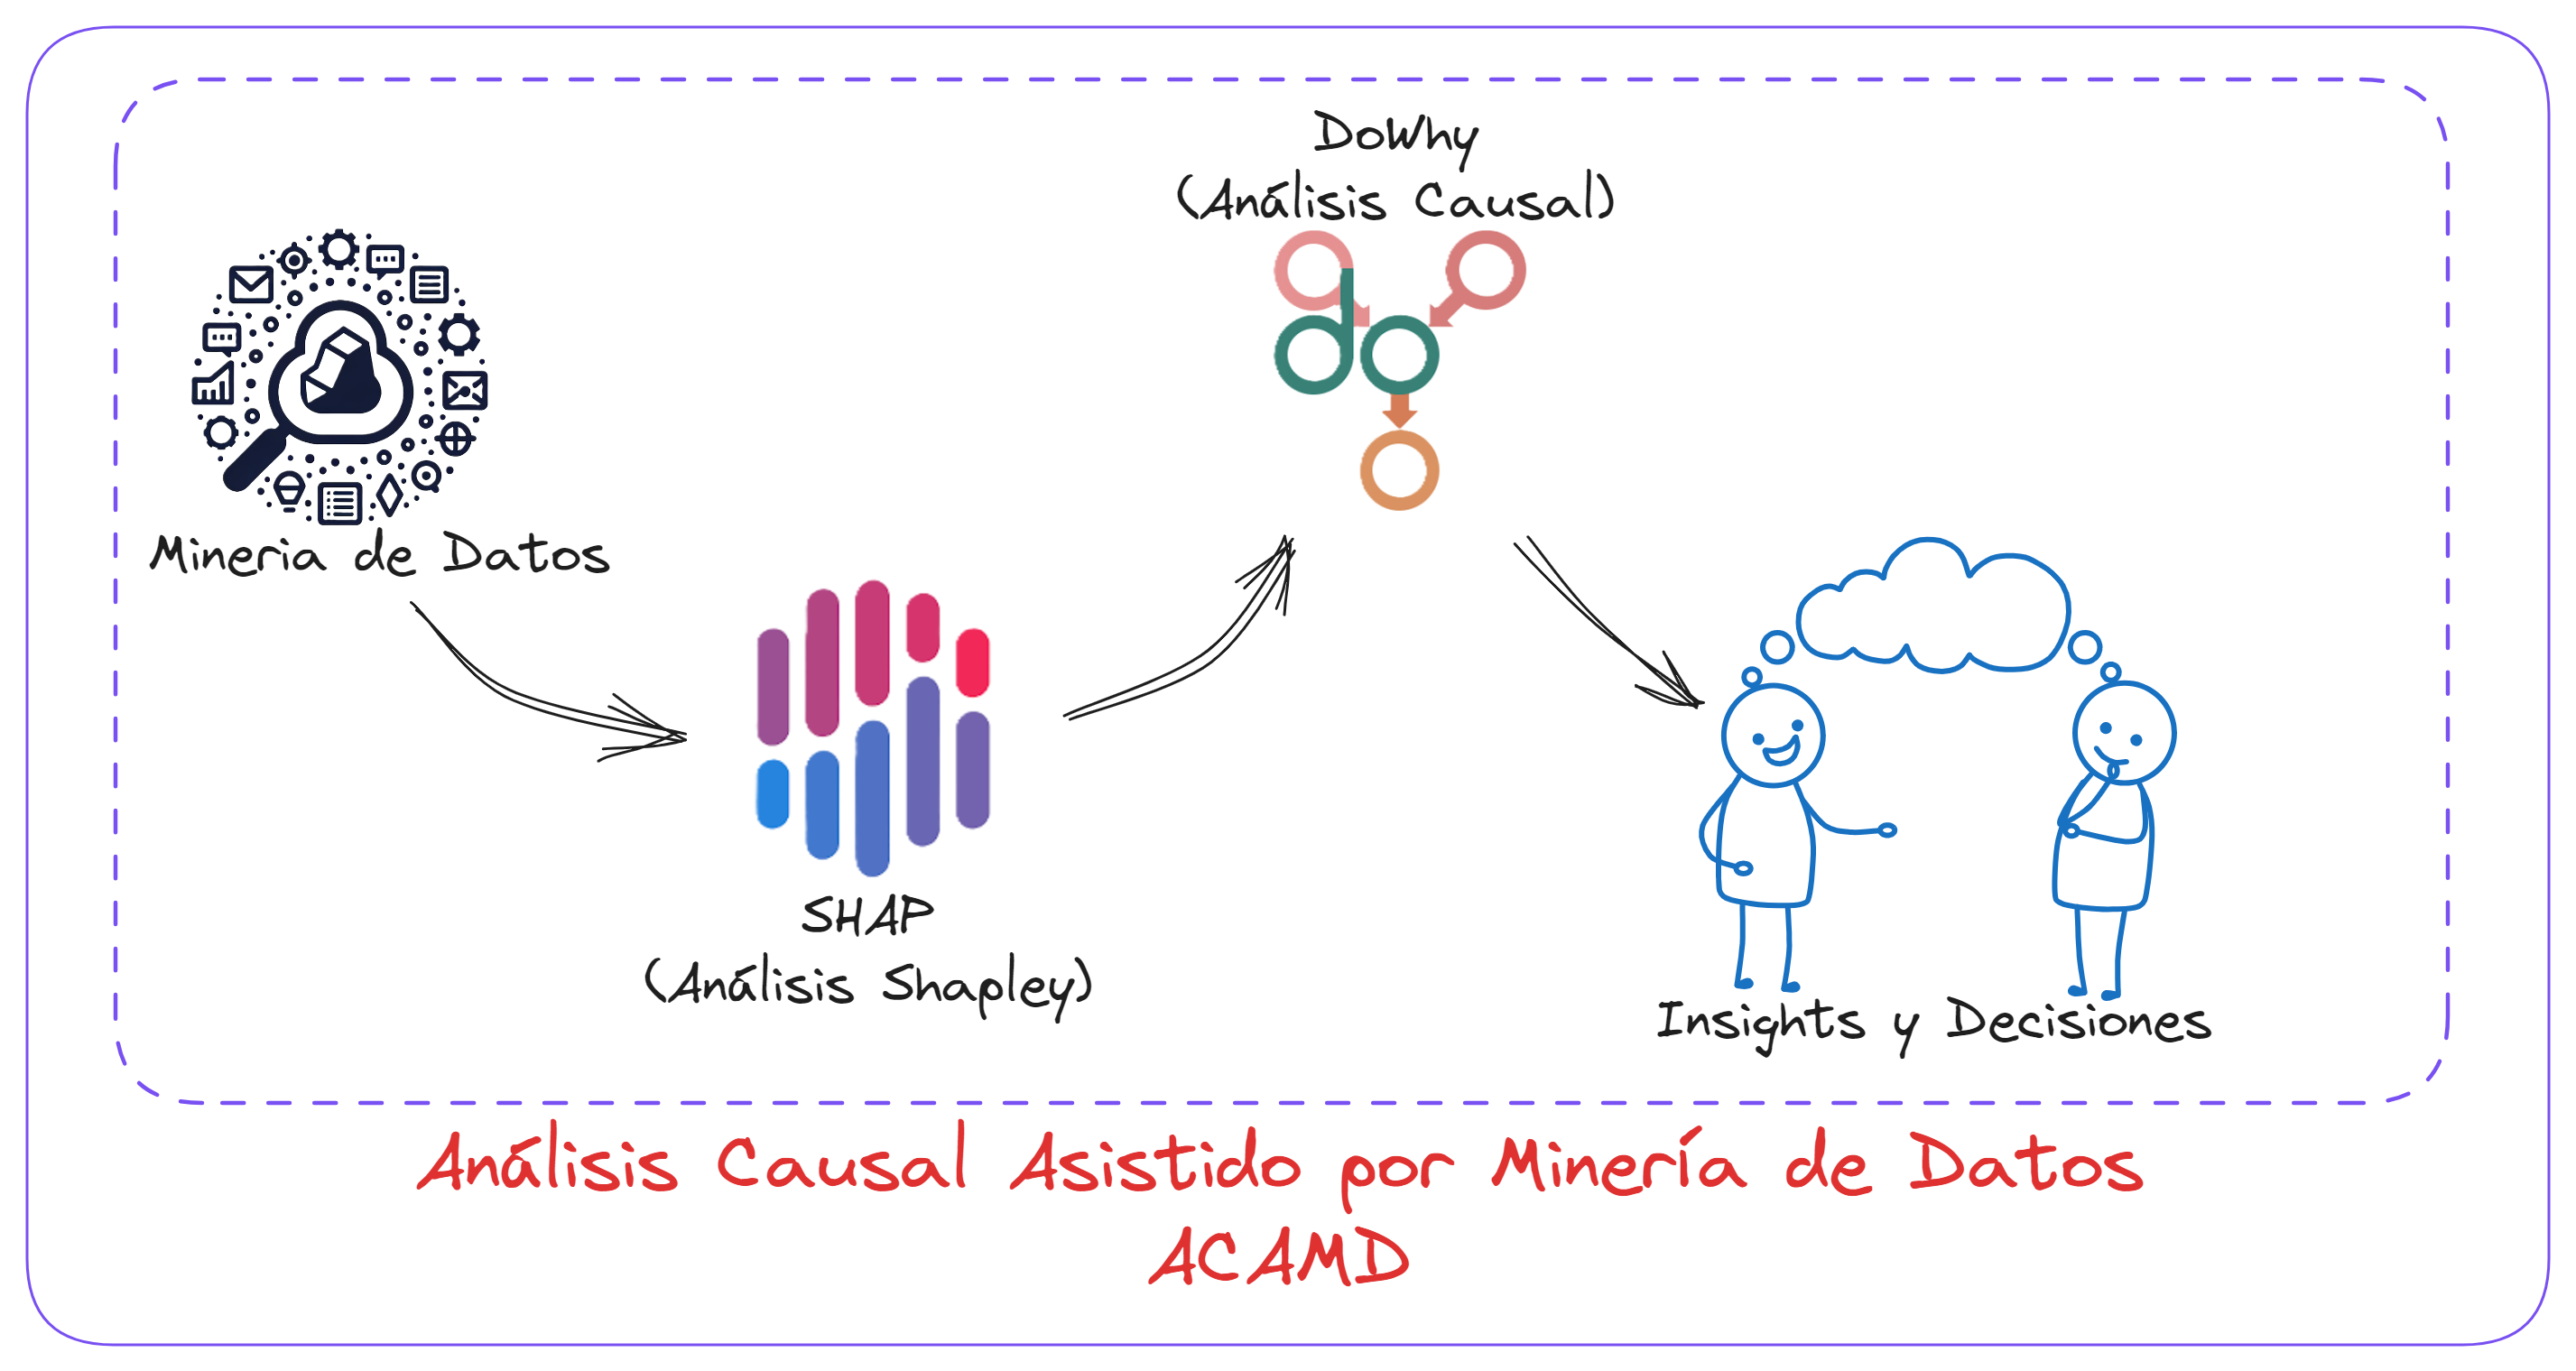
\includegraphics[width=0.7\textwidth]{img/diagramas_Tesis_ACAMD-Propuesta.png}
    \caption{Diagrama ACAMD}
    \label{fig:diagrama_ACAMD}
  \end{figure}

\subsection{Integración de la Metodología en la Investigación}\label{subsec:integracion-metodologia}

La metodología ACAMD se integra en esta investigación en varias etapas clave. Durante el análisis de resultados, SHAP identifica las variables más influyentes, que luego informan la construcción del modelo causal en DoWhy. Este enfoque integrado no solo valida la relevancia de estas variables sino que también profundiza nuestra comprensión de las relaciones causales en la investigación.

\subsection{Conclusión}\label{subsec:conclusion-metodologia}

La metodología \textit{Análisis Causal Asistido por Minería de Datos} ofrece un enfoque comprensivo y detallado para el análisis causal en el contexto de esta investigación. Al combinar las fortalezas de SHAP y DoWhy, ACAMD promete mejorar la robustez y la claridad del análisis de datos, proporcionando insights valiosos y explicaciones convincentes de los fenómenos estudiados.
